\chapter{Proposta}
  \capepigrafe[0.5\textwidth]{``Não tente se tornar uma pessoa de sucesso,
  prefira tentar se tornar uma pessoa de valor.''}{Albert Einstein}

  \section{Como criar produtos com qualidade?}
    Quando produzimos um \textit{software}, focamos sempre nas funcionalidades que
    o sistema deve conter, pretendemos entregar o mais rápido possível e respeitar
    as datas alinhadas com o negócio. Porem, na pressa de colocar as funcionalidades
    em produção, desconsideramos os requisitos não-funcionais e por mais que a
    funcionalidade tenha sido entregue conforme o específicado, o usuário não
    consegue utiliza-la, consequentemente, está entrega não está gerando valor. \newline
    Mas como assim, os requisitos foram atendidos mas o usuário não consegue utilizar?
    Como ignoramos os requisitos não-funcionais, o usuário pode estar sofrendo por
    diversos problemas, por exemplo, um \textit{layout} confuso, um desempenho baixo,
    o sistema está forçando ele a realizar uma tarefa que ele não está acostumado a
    fazer, ou pelo menos não no momento em que apareceu no sistema. Como entregamos
    vizando a data da entrega e nãp o valor para o usuário, aceitamos o risco de
    entregar algo que o usuário não vê valor, e por diversas vezes cometemos erros.
    Ao testar uma funcionalidade, não costumamos ter a visão total do negócio,
    focamos na funcionalidade, então questões como tempo de resposta, ordem lógica
    no processo, localização das informações, nos passam despercebidos, não estamos
    utilizando o sistema diariamente para entender estas questões sozinhos, e o
    negócio muda frequentemente, então quando finalmente entendemos a realidade do
    usuário, ela já mudou, e voltamos a estar sucetiveis ao erro. \newline
    Como não atendemos a expectativa do usuário, e a funcionalidade não está gerando
    valor, implementamos diversas melhorias, todas o mais rápido possível, o que
    acaba gerando \textit{bugs}, como erramos uma vez, precisamos corrigir o erro
    o mais rápido possível, o que nos faz ignorar novamente requisitos não-funcionais
    e, por sua vez, ignoramos questões de arquitetura de \textit{software} o que
    acaba deixando o sistema mais complexo, dificulta a sua manutenção, e deixa o
    sistema mais sucetível a erros. \newline
    Não queremos mais cometer estes erro, queremos cria o produto perfeito que
    será totalmente aderente ao usuário e que irá gerar valor para o negócio. \newline
    O primeiro passo para gerar um produto de qualidade, que auxilia a empresa a
    concluir os seus objetivos e que traga valor ao negócio e entender que não
    existe produto perfeito. Somos humanos, erramos constantemente, realizamos
    escolhas erradas, nos equivocamos. Para realizar uma entrega de pouco risco
    e extremamente acertiva, é necessário muito tempo de planejamento e de estudo,
    como por exemplo a construção de uma avião, ou de um prédio, ou de um
    equipamento hospitalar, este tipo de produto não pode ter falhas, pois caso
    tenha, é um risco para a vida das pessoas. Porem, nosso negócio é mais
    dinâmico, as necessidades muda com mais frequência do que as necessidades de
    um avião, se utilizarmos tanto tempo para planejar como podemos seguir as
    mudanças do negócio?

    \subsection{Assumindo riscos}
    Para conseguirmos acompanhar o negócio e gerar valor para a empresa, evemos
    escolher os riscos que vamos enfrentar. Mesmo um avião encara riscos em seu
    projeto, por isso que é implementado diversas redundancias nas funcionalidades
    mais importantes. Devemos pensar de forma semelhante, qual o objetivo do nosso
    projeto? Qual é sua funcionalidade mais importante? Quais são os riscos que
    vamos encarar? \newline
    Com base nisso, podemos focar a maior parte de nosso tempo no \textit{core}
    do produto, descobrindo o objetivo do sistema, podemos alinhar com os objetivos
    da empresa, assim gerando o retorno esperado. Para realizar o levantamento
    da funcionalidade é importante considerar o nome da funcionalidade, a sua
    importância, os objetivos em que ela vai nos auxiliar a alcançar, os riscos
    que vamos enfrentar com ela e as dependências para disponibilizar a
    funcionalidade ao usuário.

    \begin{table}[h!]
      \centering
      \begin{tabular}{|c|p{10cm}|}
        \hline
        \textbf{Funcionalidade} &
        Nome da funcionalidade que será desenvolvida. \\ \hline
        \textbf{Importância} &
        A importância que a funcionalidade representa para o negócio, separa entre
        alta, média e baixa. \\ \hline
        \textbf{Objetivos} &
        Os objetivos que está funcionalidade irá auxiliar à alcançar. \\ \hline
        \textbf{Riscos} &
        Quais os riscos que essa funcionalidade pode gerar para o negócio. \\ \hline
        \textbf{Dependências} &
        Quais são as dependências para a utilização e desenvolvimento dessa
        funcionalidade. \\ \hline
      \end{tabular}
      \caption{Definição da classificação de funcionalidaes}
      \label{Tabela:1}
    \end{table}

    Toda funcionalidade deve ter um nome que represente o que será desenvolvido
    pois, durante o desenvolvimento, é através do nome que os desenvolvedores
    vão se comunicar, sem um nome claro, que represente bem o negócio, os
    desenvolvedores não vão conseguir se comunicar de forma clara para entender
    as necessidades do negócio. Termos e nomeclaturas devem ser estabelecidas,
    para que o usuário entenda como o sistema deve ser utilizado e para os
    desenvolvedores compreenderem como o sistema será utilizado. Através desta
    comunicação, o time de desenvolvimento consegue extrair os requisitos de forma
    mais fácil e formular um padrão de qualidade. \newline
    É necessário colocar a importância da funcionalidade que será desenvolvida pois,
    com base nela podemos entender a ordem que vamos iniciar o desenvolvimento
    e quais os riscos podemos enfrentar e através da importância podemos definir
    o rigor dos testes que devemos realizar no desenvolvimento da funcionalidade
    e o padrão de qualidade para cada nível de importância. Embora colocamos
    somente três níveis de importância (alto, médio e baixo), cada negócio pode
    ter mais níveis, porém recomendamos não exagerar e passar de cinco níveis,
    pois o principal objetivo desta classificação é forçar escolhermos quais
    funcionalidades são realmente mais importantes, se colocarmos muitos níveis,
    a menor classificação será "alta". \newline
    As funcionalidades que vamos desenvolver tem que estar relacinada com um
    objetivo da empresa, pois é isso que dá propósito para ela, e a nossa base
    para verificar se ela está gerando valor. Com base no uso da funcionalidade,
    podemos verificar se o objetivo está sendo alcançado, e com base nesse
    retorno, podemos decidir quais serão os nossos próximos passos. \newline
    Quando pensamos em uma funcionalidade, devemos sempre considerar os riscos
    para o negócio, a utilização de um sistema implica em com a operação da
    empresa trabalha, e toda mudança gera riscos para a operação. Tudo que é
    novo, deve ser ensinado, por mais que a funcionalidade reflita exatamente o
    que os usuários já faziam, eles vão começar a eecutar essas atividades em
    um outro lugar, o que no começo pode gerar dúvidas e frustrações. Devemos
    sempre levantar os riscos com base na perspectiva do usuário, pois assim
    podemos entender quais serão as reações delese e quais estratégias devemos
    utilizar para engajar o uso da ferramenta e buscar por melhorias. \newline
    Com base nos objetivos, nas funcionlidades e nos riscos, podemos mapear as
    pendências das funcionalidades, onde conseguimos traçar quais os passos que
    devemos tomar para iniciar o desenvolvimento até disponibilizar a funcionalidade
    para o usuário. \newline
    Para o levantamento dessas informações recomendamos utilizar o formato de
    tabela. A tabela possibilita consolidar de forma clara cada tópico e sempre
    que a empresa tiver um novo objetivo, é mais fácil analisar o que já foi listado,
    possibilitando ver se o sistema se encaixa com essa nova necessidade ou se será
    necessário uma nova funcionalidade, ou se será necessário um novo produto,
    ou uma reformulação do negócio. Quando listamos tudo que estamos fazendo
    junto com o que o negócio pretende alcançar, podemos tomar decisões mais
    acertivas, entender dependências e otimizar o valor que será desenvolvido.
    Muitas vezes focamos em desenvolver uma funcionalidade que não irá gerar
    muito valor para o negócio, o que nos faz aceitar um risco que não precisamos
    no momento, toda funcionalidade gera riscos, então é melhor nos concentrarmos
    somente naqueles que podem gerar mais valor. \newline
    Uma vez definido nossas funcionalidade, sua importância e os objetivos que
    pretendemos com elas, podemos escolher quais vamos implementar primeiro e
    quais riscos nós vamos enfrentar. \newline
    Para exemplificar a utilização da tabela proposta vamos considerar uma
    empresa que possuí vendores que entram em contato com outras empresas para
    negociar a venda de computadores. Estes computadores podem ser customizados
    pelo cliente, solicitando maior espaço de memória, se deseja um computador
    com \textit{SSD} ou \textit{HD}, qual o processador, entre outras ecolhas.
    Embora já existam computadores pré-montados, eles podem ser customizados
    somente aproveitando a base do produto. \newline
    Hoje a venda é feita sem a utilização de um sistema, a especificação que o
    cliente deseja é feita de forma indivídual por cada vendedor e controlado por
    meio de planilhas, onde cada vendedor possui a sua forma de organizar. Somente
    o pedido final é colocado em um sistema de controle de pedidos, para emitir a
    nota. A comunicação entre os vendedores e a área técnica é feita por meio de
    telefone e email, os produtos base e os produtos vendidos são compartilhados
    através de planilhas enviadas por email. Como cada vendedor negocia de uma
    forma, nã há Padronização nas planilhas, o que acaba gera confusões na área
    técnica na hora da montagem dos produtos. Outro ponto a destacar é que a área
    administrativa não tem visibilidade de como as negociações estão sendo realizadas
    o que dificulta o entendimento do negócio como um todo e a cração de
    estratégias. \newline
    Com base nessas necessidades, a empresa decidiu começar um projeto para a
    criação de um sistema para os vendedores realizar as suas negociações.
    Onde o produto base seria disponibilizado na ferramenta e os pedidos finais
    seriam montados conforme a negociação avança. Outra necessidade, é que a
    negociação deve ser faseada, para que seja possível rastrear os passos do
    vendedor e ter uma melhor visão do negócio. \newline
    Neste cenário, o primeiro passo é levantar as princípais funcionalidades para
    atender o negócio, já colocando a sua importância e os objetivos que pretendemos
    alcançar.

    \begin{table}[h!]
      \centering
      \begin{tabular}{|c|c|p{8cm}|}
        \hline
        \textbf{Funcionalidade} &
        \textbf{Importância}  &
        \textbf{Objetivos} \\ \hline
        %Funcionalidade
        Cadastro de produtos &
        %Importância
        Alta &
        %Objetivos
        Padronização na criação de produtos; \newline
        Reduzir o cadastro incorreto de produtos.
        \\ \hline
        %Funcionalidade
        Venda de produtos &
        %Importância
        Alta &
        %Objetivos
        Venda faseada do produto; \newline
        Melhor rastreabilidade da venda; \newline
        Padronização da negociação.
        \\ \hline
        %Funcionalidade
        \textit{Chat} interno &
        %Importância
        Baixa &
        %Objetivos
        Otimização da comunicação entre a área técnica e os vendedores.
        \\ \hline
      \end{tabular}
      \caption{Exemplo de levantamento de funcionalidades}
      \label{Tabela:2}
    \end{table}

    Na tabela dois, representamos três funcionalidades, o cadastro de produtos,
    a venda de produtos, e o \textit{chat} interno. Podemos notar que a maior necessidade
    da empresa é a de padronizar a venda do produto, onde a negociação deve ser
    feita de forma mais uniforme e que facilite os vendedores a venderem produtos
    mais aderentes com o que a área técnica consegue produzir. Com base nestas
    necessidades, foi levantado as funcionalidades de cadastro de produtos e
    venda de produtos, onde o cadastro está relacionada com a padrinização da
    criação do produto e a venda está relacionada com a padronização da venda.
    Porem, a funcionalidade de \textit{chat} interno, não é uma prioridade para
    o negócio, as áreas estão se comunicando, o problema é que cada vendedor
    trabalha de um jeito, o que dificulta as decisões da área técnica. Embora um
    dos objetivos seja melhorar a comunicação entre as áreas, este não é o maior
    dos problemas que precisamos resolver, então os riscos que desta funcionalidade
    não precisam ser corridos até o desenvolvimento das outras duas. \newline
    Outro ponto de destaque é a identificação das dependências, quando mapeamos
    as dependências, conseguimos ver qual funcionalidade precisamos realizar
    primeiro, como listado no exemplo, não é possível vender os produtos sem antes
    cadastrá-los. Mas alem da dependências entre funcionalidades, podemos listar
    o que precisamos fazer para disponibilizar a funcionalidade para o usuário,
    como apresentado no exemplo, todas as funcionalidades precisam de treinamento,
    como o sistema é novo e cada vendedor realiza as negociações do seu jeito,
    é importante explicar como foi montado o processo de vendas e apresentar
    como realizar as atividades no sistema. \newline
    Cada funcionalidade tem os seus riscos, porem é através de sua importância que
    podemos criar estratégias para enfrentar estes riscos e marcar estas ações
    que definimos em nossa estratégia como dependências para liberar o uso da
    funcionalidade, é importante atrelar estas ações como dependências, pois desta
    forma os usuários não são surprendidos, e é através dos treinamentos e das
    apresentações que podemos pegar o \textit{feedback} dos usuário e começar a
    mapear novas funcionalidades e melhorias. Podemos ver o mapeamento dos riscos
    e das dependências das funcionalidades exemplo na tabela três.\newline

    \begin{table}[h!]
      \centering
      \begin{tabular}{|c|p{4cm}|p{6cm}|}
        \hline
        \textbf{Funcionalidade} &
        \textbf{Riscos}  &
        \textbf{Dependências}
        \\ \hline
        %Funcionalidade
        Cadastro de produtos &
        %Riscos
        Processo de cadastro de produtos mais demorado; \newline
        Criação de produtos menos flexível. &
        %Dependências
        Treinamento para cadastrar os produtos no sistema;\newline
        Explicação das regras utilizadas para o cadastro dos produtos.
        \\ \hline
        %Funcionalidade
        Venda de produtos &
        %Riscos
        Venda menos flexível; \newline
        Mudança na forma de negociação dos vendedores; &
        %Dependências
        Funcionalidade de cadastro de produtos; \newline
        Treinamento para realizar vendas no sistema; \newline
        Explicação das fases na venda.
        \\ \hline
        %Funcionalidade
        \textit{Chat} para clientes &
        %Riscos
        Não adoção do \textit{chat} como princípal meio de comunicação; \newline
        Utilização do \textit{chat} para assuntos sem relação ao trabalho; &
        %Dependências
        Treinamento para a utilização do \textit{chat}; \newline
        Treinamento sobre como se comunicar por \textit{chat}.
        \\ \hline
      \end{tabular}
      \caption{Exemplo de levantamento dos riscos e dependências por funcionalidade}
      \label{Tabela:3}
    \end{table}

    \subsection{Entendendo os requisitos de uma funcionalidade}
    Após entendermos os ricos, escolher quais vamos aceitar e definir a prioridade
    das funcionalidades que queremos desenvolver, devemos começar a refinar cada
    uma e definir quais são seus requisitos. É importante salientar que os
    requisitos, assim como foi com os riscos, devem partir do negócio, para assim
    fazer parte do sistema, a funcionalidade deve solucionar um problema e facilitar
    a vida dos usuários, agregando valor para o cotidiano deles e consequentemente
    agregando valor para o negócio. \newline
    A funcionalidade deve ser desenvolvida com base no que os usuários já fazem
    no dia a dia, temos que mapear todas as tarefas que o usuário executa,
    identificando quais incomodam e quais não incomodam. Identificando quais tarefas
    o usuário não gosta de fazer, já é um ponto de partida no que o sistema
    automatizar, uma vez que o usuário não precise fazer determinada funcionalidade,
    já facilitou o seu cotidiano. Outro ponto de atenção, são com as tarefas que
    o usuário não se importa em executar, automatizar ou mudar a forma que ele
    executa pode ser um problema em um promeiro momento, pois ele terá que se
    acostumar com uma nova forma de trabalho. Muitas vezes esse tipo de mudança
    pode se originar em uma nova fase da empresa, que está revendo os seus processos
    e mudando a forma como de trabalho dos colaboradores, neste caso, é importante
    implementar a funcionalidade de forma que seja um meio termo entre o que os
    usuários realizavam e a nova forma da empresa, desta forma os usuários
    começam a se adaptar a nova perspectiva e conforme o projeto for avançando,
    podemos ir adaptando a funcionalidade a restruturação da empresa. Devemos
    lembrar que nenhuma mudança acontece do dia para a noite, e uma mudança
    brusca na forma de trabalho pode gerar desconforto nos usuários e deixar eles
    confusos em como executar suas atividades. \newline
    Uma funcionalidade deve sofrer melhorias constantes, como o negócio está
    constantemente sofrendo mudanças, o sistema deve se adaptar para os novos
    requisitos do mercado, por este motivo, os requisitos devem ser identificados
    mas não podem ser considerados como certeza, o sistema deve estar pronto para
    sofrer qualquer tipo de alterações e a qualquer hora porem, sabemos que certas
    mudanças levam muito tempo e até a alteração, o requisito já sofreu mais uma
    alteração, por este motivo, devemos classificar nossos requisitos em nível
    de importância e em nível de mutabilidade. Enquanto nos riscos nós classificamos
    a funcionalidade como um todo, aqui vamos classificar os requisitos que formam
    essa funcionalidade, devemos sempre pensar, o que é essencial para a funcionalidade
    atingir o objetivo? O que pode se tornar uma melhoria para o futuro? Desta
    forma, conseguimos entregar valor mais rápido para diferentes áreas do negócio,
    pois se focarmos todo o nosso tempo na funcionalidade mais importante, nunca
    vamos realizar as outras funcionalidades. Para cada funcionalidade devemos
    tambem atribuir um nível de mutabilidade, ou seja, qual é a chance dessa
    funcionalidade sofrer alterações conforme o tempo vai passando, embora o
    negócio esteja em constante mudança, sabemos que certos processos dificilmente
    sofrem alterações, pois faz parte do \textit{core} da empresa, é a essência
    do negócio. A forma de classificar a mutabilidade é através de porcentagem,
    onde as primeiras classificações serão intuições com base na perspectiva do
    negócio, mas as seguintes, é importante que conforme o sistema vá sofrendo
    alterações e melhorias, estas taxas sejam atualizadas por funcionalidade.
    A primeira regra na hora de classificar é que não existe zero porcento, toda
    funcionalidade pode sofrer alterações, mesmo que demore anos para isso acontecer,
    a sociedade muda, novas tecnologias vão surgindo e o que era comum é subtituido
    por algo novo, que acaba se tornando o novo comum, e se a empresa não estiver
    preparada para acompanhar essas mudanças, ela acaba se perdendo no tempo.
    Realizando essa classificação podemos identificar quais processos estão
    consolidados e quais processos ainda devem ser estruturados, com essa visão
    sobre os processos, podemos identificar o novo \textit{core} do negócio e
    desta forma trabalhar em uma tranformação na empresa para atender as novas
    necessidades do mercado, assim evoluindo o sistema ou até mesmo desenvolvendo
    um novo, garntindo que a empresa se mantenha sempre atualizada com as tendências
    do mercado. Na tabela quatro está os atributos que devem ser levados em conta
    quando calssificarmos um requisito.\newline

    \begin{table}[h!]
      \centering
      \begin{tabular}{|c|p{10cm}|}
        \hline
        \textbf{Funcionalidade} &
        Nome da funcionalidade que o requisito faz parte. \\ \hline
        \textbf{Requisito} &
        Nome do requisito que faz parte da funcionalidade. \\ \hline
        \textbf{Importância} &
        O nível de importância do requisito separado em baixo, médio e alto. \\ \hline
        \textbf{Mutabilidade} &
        O quanto este requisito pode sofrer alterações em porcentagem. \\ \hline
        \textbf{Stakeholders} &
        Quais áreas são impactadas com esta funcionalidade. \\ \hline
        \textbf{Descrição} &
        A descrição do requisito da funcionalidade. \\ \hline
      \end{tabular}
      \caption{Definição da classificação de requisitos}
      \label{Tabela:4}
    \end{table}

    Agora que temos mapeado os processos que fazem parte de determindada funcionalidade,
    e sabemos como classificar, podemos começar a levantar eles. Todo requisito
    deve possuir uma descrição, algo que instrua o time de desenvolvimento a entender
    o seu propósito e auxilie eles a desenvolver a funcionalidade. Quando analisamos
    um requisito, outros requisitos vão surgindo pois, a um primeiro momento,
    quando levantamos os requisitos, ficamos sempre na funcionalidade, e como o
    sistema deve se comportar mas alem de estrutrar como determinada funcionalidade
    deve se comportar, devemos utilizar os requisitos como forma de garantir a
    qualidade do que será desenvolvido. É atrvés de como os usuários vão utilizar
    o sistema que podemos identifcar o que precisamos garantir que funcione durante
    a utilização do usuário. Questões como quantidade de acessos, tempo de resposta,
    usabilidade, métricas, devem ser consideradas como requisitos do sistema, algo
    diretamente realcionado ao que vai ser desenvido e estabelcer um critério de
    aceitável ou não para a utilização em produção. Quando identificamos os requisitos
    devemos tambem identificar quais áreas da empresa será impactada pelo requisito.
    Para os requisitos funcionais, devemos identificar quais são as áreas que vão
    utilizar esta funcionalidade, para os requisitos não-funcionais, identificamos
    as áreas que caso o requisito não seja atendido, serão impactadas, caso o
    requisito não seja atendido, quais áreas terão seu processo afetado, podendo
    criar um bloquio ou deixando ele mais longo. Para exemplificar o levantamento
    dos requisitos, vamos utilizar a funcionalidade de "Cadastro de produtos",
    utilizado no exemplo de identificação dos riscos. \newline
    Para realizar o cadastro de produtos, vamos supor que envolva três áreas, o
    \textit{marketing}, a equipe técnica e vendas. A equipe de \textit{marketing},
    com base em suas análises de mercado e nas solicitações dos vendedores, analisam
    as tendências dos pedidos do cliente e montam projetos para novos produtos,
    este projeto é enviado para a área técnica que avalia se é viável ou não a
    sua execução, podendo aprovar ou recusar a montagem desse produto. Caso o
    produto o seja recusado, o solicitação é devolvida para a equipe técnica,
    com os motivos da recusa, onde eles podem realizar as devidas alterações ou
    cancelar o projeto. Caso seja aceito, a equipe técnica começa a montagem,
    realizam seu testes e validam se está aderente com o que foi proposto no
    projeto, uma vez encerrado está etapa, é anunciado aos vendedores que há um
    novo produto no catálogo e caso tenha relação à algum pedido de algum vendedor,
    ele é notificado que determinado produto foi produzido. Há casos, em que o
    vendedor pega um produto base e este deve ser customizado com base nas
    especificações do cliente. \newline

    \begin{table}[h!]
      \centering
      \begin{tabular}{|c|p{10cm}|}
        \hline
        \textbf{Funcionalidade} &
        Cadasto de produtos \\ \hline
        \textbf{Requisito} &
        Notificação de projeto de produto base \\ \hline
        \textbf{Importância} &
        Média \\ \hline
        \textbf{Mutabilidade} &
        45\% \\ \hline
        \textbf{Stakeholders} &
        Área técnica \\ \hline
        \textbf{Descrição} &
        Quando um projeto de produto base for cadastrado, o sistema deve
        enviar uma notificação para a área técnica, que um novo produto
        foi cadastrdo e agurda aprovação. \\ \hline
      \end{tabular}
      \caption{Exemplo de classificação de requisito funcional}
      \label{Tabela:5}
    \end{table}

    \begin{table}[h!]
      \centering
      \begin{tabular}{|c|p{10cm}|}
        \hline
        \textbf{Funcionalidade} &
        Cadasto de produtos \\ \hline
        \textbf{Requisito} &
        A notificação deve ser enviada imediatamente para a área técnica \\ \hline
        \textbf{Importância} &
        Média \\ \hline
        \textbf{Mutabilidade} &
        10\% \\ \hline
        \textbf{Stakeholders} &
        \textit{Marketing}, área técnica \\ \hline
        \textbf{Descrição} &
        A notificação da criação do projeto deve ser enviada em um intervalo de
        menos de um segundo para a área técnica. \\ \hline
      \end{tabular}
      \caption{Exemplo de classificação de requisito não-funcional}
      \label{Tabela:6}
    \end{table}

    \begin{table}[h!]
      \centering
      \begin{tabular}{|c|p{10cm}|}
        \hline
        \textbf{Funcionalidade} &
        Cadasto de produtos \\ \hline
        \textbf{Requisito} &
        O cadastro é destinado somente para produtos base \\ \hline
        \textbf{Importância} &
        Alta \\ \hline
        \textbf{Mutabilidade} &
        7\% \\ \hline
        \textbf{Stakeholders} &
        Vendas \\ \hline
        \textbf{Descrição} &
        Os produtos que serão cadastrados nesta funcionalidade deve somente ser
        somente produtos base, customizações serão feitas na venda do prostudo. \\ \hline
      \end{tabular}
      \caption{Exemplo de classificação de requisito inverso}
      \label{Tabela:7}
    \end{table}

    Embora a funcionalidade de "Cadastro de produtos" tanham muitos outros requisitos,
    vamos exemplificar somente os que estão nas tabelas cinco, seis e sete.
    O requisito da tabela cinco se trata de um requisito funcional, o requisito de
    enviar a notificação para a área técnica quando um projeto for criado. Podemos
    notar que sua mutabilidade é média, embora o processo dificilmente possa mudar,
    a área técnica sempre deve ser informada quando um projeto for criado pois,
    são eles que aprovam se o projeto é válido ou não porem, no futuro é possível
    que seja criada uma nova área somente para análise de projetos, hoje está
    concentrado dentro da mesma área que monta o produto, outra alteração é a
    adição de outra área, hoje o negócio esntende que somente a área técnica deve
    ser informada porem, os vendedores tambem fazem parte do processo, uma vez que
    o projeto pode se tratar de uma solicitação deles, por este motivo, a área de
    vendas pode ser incluída no recebimento da requisição. Embora os vendedores
    tambem participem desse processo, a notificação é destinada somente para a área
    técnica, desta forma, somente a else são um \textit{stakeholder} desse
    requisito. Na tabela seis, temos um requisito não-funcional, é um requisito
    que está atrelado diretamente a qualidade da fincionalidade, ela está definindo
    que a notificação deve ser disparado com no máximo um \textit{delay} de um
    segundo da criação do produto. Para o negócio é importante que a área seja
    informada que um novo projeto foi criado imediatamene após sua criação, este
    requisito deve ser utilizado como critério de qualidade e utilizado como cenário
    de teste, não somente da criação de um projeto, mas para a criação de vários
    projeto de uma vez só. Na tabela sete, possuímos um requisito inverso, algo
    que o sistema não deve fazer, que no caso, é que a funcionalidade de "Cadastro
    de produtos" se destina somete para produtos base, ou seja, as customizações
    dos vendedores não estão incluidas nessa funcionalidade, é interessante na
    descrição deste requisito, sempre colocar em qual funcionalidade este requisito
    se aplica, caso ele se aplique a alguma funcionalidade. Como a customização
    dos produtos base está sempre atrelada a venda do produto e não ao seu
    cadastro, podemos ver que dos tês exemplos, este é o de menor mutabilidade,
    pois este processo dificilmente será mudado e atribuir a responsábilidade ao
    vendedor de cadastrar um produto, somente por causas das customizações é uma
    mudança muito grande no processo de como é realizada a venda.

    \subsection{Arquitetura evolutiva}
    Conforme o produto vai evoluindo, mudanças deverão ser feitas para acompanhar
    as necessidades do negócio e para isso, devemos construir o nosso sistema de
    forma que seja fácil implementar novas funcionalidades e aplicar mudanças e
    melhorias em funcionalidades já desenvolvidas. Para que isso seja possível,
    devemos desenvolver um \textit{software} com alto nível de abstração, cada
    parte do sistema deve funcionar de forma quase indivídual, para que desta
    forma uma alteração realizada em alguma parte do sistema, não afeta as demais
    e assim, minizamos \textit{bugs} e tempo de manutenção e desenvolvimento de
    melhorias. \newline
    O mundo perfeito, realmente é desenvolver um sistema como o descrito anteriormente,
    com alto nível de abstração e cada parte do sistema funcionando de forma indivídual,
    mas para montar determindado sistema, é necessário que o produto e a equipe
    de desenvolvimento esteja extremamente madura, no começo do projeto ainda não
    sabemos quais são as partes do sistema, não conseguimos separar o que deve
    funcionar de forma indívidual e o que faz parte desse indívidual. Para
    descobrirmos é importante quando desenharmos a arquitetura de nosso sistema,
    nos atentarmos na mutabilidade de cada requisito, devemos desenvolver cada
    funcionalidade como se ela pudesse mudar a qualquer hora, mas quando tivermos
    que tomar a decisão em qual parte deverá ficar mais abstraída do sistema,
    a mutabilidade dos requisitos deverá ser considerada. Com base na mutabilidade,
    podemos montar a base de nosso sistema, as funcionalidades que muito dificilmente
    deverão ser modificadas, e a partir delas evoluir o sistema para as outras
    funcionalidades, que dependendo do nível de mutabilidade, deverá funcionar de
    forma quase independente, desta forma, conforme o tempo for passando, podemos
    ir isolando as partes do sistema cada vez mais, a medida que a mutabilidade
    dos requisitos vão ficando mais acertivas com a realidade e novos requisitos
    vão surgindo, pois desta forma, a equipe de desenvolvimento terá um melhor
    entendimento do negócio e conseguirá abstrair o sistema de forma mais condizente
    de como o negócio funciona. \newline
    Após tivermos um sistema extremamente abstraído e um time de desenvolvimento
    com um grande entendimento do negócio, podemos evoluir nossa arquitetura para
    microserviços, de forma que, cada parte do sistema é verdadeiramente um sistema
    apartado, com seu próprio time e requisitos, onde todas essas funcionalidades
    se encontram na mesma plataforma. Quando conseguimos evoluir nosso produto
    para este nível, ele deixa de ser um sistema para se tornar uma plataforma,
    um lugar onde vários sistemas vão ser executado para cumprir diversos Objetivos
    relacionados. Lembrando, que embora agora temos vários sistemas, realizando
    diversas tarefas diferentes, o objetivo da plataforma deve ser o mesmo de
    quando iniciamos o projeto, nunca devemos esquecer o objetivo do produto ter
    sido criado, porque é com base nele que as melhorias e os requisitos devem ser
    levanrados, uma vez que esqucemos desse objetivo, nosso produto começa a
    realizar diversas ações que não estão relaciondas, sua arquitetura fica cada
    vez mais complexa e nosso produto perde seu propósito. \newline
    Uma vez que nosso produto esteja separado em vários sistemas, podemos reaproveitar
    as funcionalidades que desenvolvemos em outros produtos, e como cada sistema
    da plataforma tem a sua própria equipe, as análises realizadas no produto
    serão realizdas em cada parte de valor do que foi desenvolvido, com esses
    dados, podemos analisar qual parte do negócio está sofrendo maior alteração,
    qual está gerando mais valor, qual precisa ser reestruturada, qual precisa
    de mais investimento, quais áreas podem ser dividas, entre outras. Como
    cada parte da nossa plataforma está se preocupando com uma determindada parte
    do negócio e como, nosso time já conseguiu separar essas partes de uma forma
    que esteja completamente aderente a como o negócio funciona, conseguimos ter
    a visão de todas as atuações da empresa no mercado. Conseguimos ter a visão
    do todo separada em várias equipes diferentes, preocupadas em evoluir a sua
    parte e contribuir com as outras. Com essa visão, podemos evoluir nossos
    sistemas para outras plataformas, com objetivos diferentes, e agregrando
    valor para o negócio de forma distinta. Podemos através das necessidades do
    mercado, e com os requisitos do sistema, reformular a forma que a empresa
    atua no mercado, identificar atuações secundárias da empresa, que tem potencial
    para se tornar primárias, fazer os sócios e diretores enxergarem cada pedaço
    que gera valor para a empresa e definir estratégias não tradicionais, algo
    diferente, para adquirir uma possível vantagem no mercado.

    \subsection{Estruturando o fluxo de entrega}
    Para alcançarmos nossos objetivos e desenvolvermos as nossas funcionalidades
    em tempo ágil, com qualidade e se preocupando em manter nossa arquitetura
    simple e evolutiva, precisamos estruturar o nosso fluxo de entrega, ou seja,
    precisamos definir como será o processo de desenvolvimento, verificação de
    qualidade, homologação e subida em produção. \newline
    Para cada requisito, devemos escrever os critérios de aceite, para que eles
    sejam considerados cumpridos, para que desta forma, quem for testar as
    funcionalidades, consigam compreender o que devem verificar e para que os
    desenvolvedores, compreendam como devem desenvolver a funcionalidade. Desta
    forma, alem de termos desenvolvedores e testadores cientes de como deve
    o sistema deve funcionar, conseguimos criar um padrão de qualidade, que será
    documentado e revisado conforme o produto for evoluindo pois, conforme o tempo
    for passando, novos requisitos forem surgindo e os requisitos já mapeados
    forem mudando. Com os critérios de aceite escritos, podemos mapear quais
    testes deverão ser feitos para cada funcionalidade, teste de regressão, teste
    de fumaça, teste de integração, teste em massa, teste unitário, cada requisito
    vai exigir um determindao tipo diferente de teste, e com o critério de aceite
    é importante mapearmos não somente quais testes, mas tambem em quais cenários
    e como eles devem ser executados, pois é nos testes que devemos procurar simular
    os momentos mais importantes para o negócio, os momentos em que o sistema não
    pode falhar. Embora cada requisito tenha o seu próprio conjunto de testes,
    é importante padronizar que todas as novas funcionalidades tenham sempre testes
    unitários e em massa, e para melhorias ou mudanças seja sempre realizado testes
    de regressão, caso uma nova funcionalidade esteja relacionada com outra, é
    importante tambem realizar os testes de regressão nas funcionalidades
    relacionadas. Os critérios de aceite devem ser escritos se baseando diretamente
    nos riscos que aceitamos, quando mapeamos as funcionalidades, nossos testes,
    alem de garantir que os requisitos da funcionalidade sejam cumpridos, deve
    direcionar os nossos testes para que realizemos as situações que mapeamos como
    risco, embora os riscos tenham sido aceite, precisamos verificar como o sistema
    vai se comportar nestes cenários, desta forma conseguimos antes de disponibilizar
    para o usuário, averiguar se realmente faz sentido correr esse risco ou não. \newline
    Para exemplificar a escrita dos critérios de aceite, vamos utilizar o requisito
    da tabela seis. \newline

    \begin{table}[h!]
      \centering
      \begin{tabular}{|c|p{10cm}|}
        \hline
        \textbf{Funcionalidade} &
        Cadasto de produtos \\ \hline
        \textbf{Requisito} &
        A notificação deve ser enviada imediatamente para a área técnica \\ \hline
        \textbf{Critério} &
        Deve ser disparado a notificação para todos os produtos que forem criados. \\ \hline
        \textbf{Critério} &
        Na notificação deve conter o nome do produto e quando ele foi criado. \\ \hline
        \textbf{Critério} &
        A área técnica deverá identificar se uma notificação já foi lida ou não. \\ \hline
        \textbf{Critério} &
        A notificação somente deve ser marcada como lida caso o usuário da área
        técnica acesse a notificação. \\ \hline
      \end{tabular}
      \caption{Exemplo de especificação de critérios de aceite}
      \label{Tabela:8}
    \end{table}

    Na tabela oito, podemos verificar os critérios de aceite para o requisito de
    notificação da funcionalidade de "Cadastro de produtos". Podemos notar que cada
    requisito descreve como a funcionalidade deve funcionar, assim como auxilia
    como este requisito deve ser testado, conseguimos identificar tambem que este
    requisito deve ser testado de forma massiva, pois um dos critérios é de que
    cada produto deve disparar obrigatóriamente uma notificação, desta forma, se
    eu criar nove produtos de uma vez, deve ser gerada uma notificação para os
    nove produtos. \newline
    Agora que definimos como nosso requisito será desenvolvido e como ele será
    testado, precisamos definir em qual momento cada uma dessas ações deverá ser
    realizada e em qual ambiente. Quando estamos desenvolvendo uma funcionalidade
    devemos sempre testar ela por completo, mas para sermos ágeis, não podemos
    esperar todos os requisitos serem desenvolvidos para iniciarmos os testes,
    da mesma forma que os desenvolvedores não podem ficar aguardando todos os
    testes serem realizados para iniciarem um novo desenvolvimente. Enquanto os
    testadores só podem iniciar um teste assim que um desenvolvedor finalizar
    uma atividade e os desenvolvedores não podem alterar a funcionalidade para não
    influenciar nos testes, é interessante realizar estas ações em ambientes
    separados. Os desenvolvedores realizam os seus desenvolvimento em um ambiente
    exclusivo para desenvolvimento, enquanto os testadores realizam seus testes
    em um ambiente exclusivo para testes. Cada critério, cada cenário deverá ser
    simulado neste ambiente, devido a isso a qualidade dos dados deste ambiente
    deverá ser o mais fiel possível ao que os usuários irão utilizar, por outro
    lado, os desenvolvedores necessitam de dados somente para verificar se a
    funcionalidade está funcionando e os critérios foram atendidos, devido a isso,
    é importante ter uma boa qualidade nos dados, mas não é preciso investir
    tanto tempo nos dados deste ambiente. Vamos chamar o ambiente dos desenvolvrdores
    de \textbf{DEV} (desenvolvimento) e o ambiente dos testadores de \textbf{QA}
    (\textit{Quality Assurance}). \newline
    Os desenvolvedores tem a obrigação de garantir que todos os critérios do
    requisito desenvolvido seja atendido, ou seja, só é permitido disponibilizar
    o requisito para ser testado no ambiente de \textbf{QA} após o desenvolvedor
    testar todos os crtérios no ambiente de \textbf{DEV}. O requisito disponibilizado
    em \textbf{QA}, o testador deverá testar todos os critérios nos mais diversos
    cenários possíveis, dando foco nos riscos que foram mapeados na especificação
    do requisito e conforme mais requisitos vão sendo disponibilizados, ele deverá
    testar novamente todos cenários novamente, mas agora validando os critérios
    dos outros requisitos. Desta forma, conseguimos garantir que as situações de
    maior necessidade do negócio está sendo contemplada. Para que possamos gerar
    valor de forma ágil, é importante que na primeira iteração do time, seja
    desenvolvida somente as funcionalidades de maior importância, pois dessa
    forma conseguimos integrar uma funcionalidade de forma rápida, embora ela
    realizando o minimo planejado, já podemos como será a reação dos usuários e
    identificar se há a necessidade de mudanças ou melhorias para serem desenvolvidas
    na próximas iteração, além de reavaliar a importância dos requisitos mapeados. \newline
    Logo após todos os testes em todos os cenários de risco da funcionalidade,
    podemos disponibilizar a funcionalidade para homologação, ou seja, devemos
    realizar todas as atividades que o usuário irá executar, com o objetivo de
    verificar se o que foi desenvolvido está aderente com o negócio, podemos
    tambem realizar apresentações para os usuários, afim de adiantar para eles
    o que será entregue e preparar uma documentação de como determinada funcionalidade
    funciona, com o intuíto de disponibilizar esta informação para os usuários e
    para novos integrantes do projeto. Todo esse processo deve ser realizado em
    um ambiente separado que vamos nomear de \textbf{HOMOL} (homologação). Este ambiente deve
    estar separado pois os dados que contem nele, devem ser preparados para
    apresentações, como ele será utilizado para compreender o que será entregue
    para o usuário e para apresentar uma prévia para eles, as funcionalidades
    não devem ser influênciadas por funcionalidades em desenvolvimento e os
    dados presente nelas, não devem ser influênciadas pelos testes realizados
    pelos testadores. Os dados neste ambiente deve ser o mais limpo possível,
    ele deve ser o mais próximo possível do que os usuários irão utilizar em
    produção, e as funcionalidades que estão neste ambiente devem estar completamente
    testadas e com todos os critério garantidos. \newline
    Após realizarmos a homologação da nossa funcionalidade, devemos nos preparar
    para entregar essa funcionalidade para os usuários, para isso, vale realizarmos
    uma ultima validação, em um ambiente que vamos nomear de \textbf{PREPROD}
    (pré-produção). Este ambiente deve ser uma cópia perfeita de produção, nele
    devemos realizar novamente todos os princípais testes que já realizamos em
    \textbf{QA} e \textbf{HOMOL}, para verificar que todos os critérios continuam
    sendo cumpridos, alem de aplicarmos treinamentos para os usuários da nova
    funcionalidade, permitindo que eles utilizem esta funcionalidade de forma
    controlada, para que eles aprendam a utilizar o sistema antes de colcoar ele
    no ar. Com essa abordagem, antes de disponilizar o sistema em produção,
    conseguimos verificar a reação deles com o que será entregue, alem de ter uma
    prévia de como o sistema será utilizado, desta forma já conseguimos identifcar
    melhorias para as próximas iterações. \newline

    \begin{figure}[!h]
      \centering
      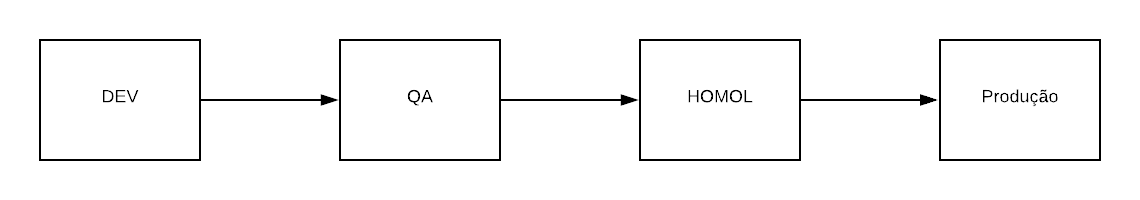
\includegraphics[width=15cm]{enviromentStream.png}
      \caption{Fluxo de ambientes}
      \label{Imagem:1}
    \end{figure}

    \subsection{Automatizando testes de qualidade}

  \section{Como adquirir escalabilidade?}
    \subsection{Descobrindo os limites do sistema}
    \subsection{Desenvolvendo estratégias de escalabilidade}

  \section{Como manter o sistema disponível?}
    \subsection{Utilizando o negócio para definir disponibilidade}
    \subsection{Analisando o desempenho do sistema}
    \subsection{Falando com os usuários}
    \subsection{Utilizando métricas para assegurar a disponibilidade}
    \subsection{Aplicando testes automatizados}

  \section{Como identificar falhas?}
    \subsection{Sentindo o cheiro do produto}
    \subsection{Utilizando o usuário para identificar falhas}
    \subsection{Solucionando falhas}
    \subsection{Aprendendo com os erros}
    \subsection{Testes automatizados como ferramenta de aprendizado}
    \subsection{Divulgando as descobertas de forma global}
